\section{细胞的DPD模型和模拟}
\subsection{红细胞的DPD模型和模拟}
\begin{frame}
\frametitle{红细胞膜结构}
\note{\textcolor{red}{330-350s}}
\note[item]{另一方面, 我们还对红细胞的运动与变形进行了模拟}
\note[item]{图8是血红细胞的模结构, 红细胞膜主要由双分子层, 跨膜蛋白及膜下的血影蛋白网组成. 血影蛋白网是细胞的主要骨架}
\begin{figure}[!htb]
\centering
\begin{tikzpicture}[scale=0.7]
\foreach \xf/\yf/\xs/\ys in {
2.9900/5.0400/2.9900/5.0400,
 2.9900/5.0400/4.7900/5.1000,
 2.9900/5.0400/1.3800/3.3900,
 2.9900/5.0400/3.6300/3.7100,
 4.7900/5.1000/4.7900/5.1000,
 4.7900/5.1000/6.9100/5.1300,
 4.7900/5.1000/3.6300/3.7100,
 4.7900/5.1000/5.7100/3.7300,
 6.9100/5.1300/6.9100/5.1300,
 6.9100/5.1300/8.6400/5.0900,
 6.9100/5.1300/5.7100/3.7300,
 6.9100/5.1300/7.9100/3.8600,
 8.6400/5.0900/8.6400/5.0900,
 8.6400/5.0900/10.8100/5.3100,
 8.6400/5.0900/7.9100/3.8600,
 8.6400/5.0900/9.5200/3.8800,
10.8100/5.3100/10.8100/5.3100,
10.8100/5.3100/9.5200/3.8800,
10.8100/5.3100/11.8700/3.7700,
 1.3800/3.3900/1.3800/3.3900,
 1.3800/3.3900/3.6300/3.7100,
 1.3800/3.3900/2.8900/2.1000,
 3.6300/3.7100/3.6300/3.7100,
 3.6300/3.7100/5.7100/3.7300,
 3.6300/3.7100/2.8900/2.1000,
 3.6300/3.7100/4.8100/2.0100,
 5.7100/3.7300/5.7100/3.7300,
 5.7100/3.7300/7.9100/3.8600,
 5.7100/3.7300/4.8100/2.0100,
 5.7100/3.7300/6.9600/2.4900,
 7.9100/3.8600/7.9100/3.8600,
 7.9100/3.8600/9.5200/3.8800,
 7.9100/3.8600/6.9600/2.4900,
 7.9100/3.8600/8.6800/2.2300,
 9.5200/3.8800/9.5200/3.8800,
 9.5200/3.8800/11.8700/3.7700,
 9.5200/3.8800/8.6800/2.2300,
 9.5200/3.8800/10.9100/2.4600,
11.8700/3.7700/11.8700/3.7700,
11.8700/3.7700/10.9100/2.4600,
11.8700/3.7700/12.9800/2.1000,
 0.5400/2.3900/0.5400/2.3900,
 1.3800/3.3900/1.6400/0.5100,
 2.8900/2.1000/2.8900/2.1000,
 2.8900/2.1000/4.8100/2.0100,
 2.8900/2.1000/1.6400/0.5100,
 2.8900/2.1000/3.8300/0.4100,
 4.8100/2.0100/4.8100/2.0100,
 4.8100/2.0100/6.9600/2.4900,
 4.8100/2.0100/3.8300/0.4100,
 4.8100/2.0100/5.6700/0.5300,
 6.9600/2.4900/6.9600/2.4900,
 6.9600/2.4900/8.6800/2.2300,
 6.9600/2.4900/5.6700/0.5300,
 6.9600/2.4900/7.8100/0.9900,
 8.6800/2.2300/8.6800/2.2300,
 8.6800/2.2300/10.9100/2.4600,
 8.6800/2.2300/7.8100/0.9900,
 8.6800/2.2300/9.6900/0.6600,
10.9100/2.4600/10.9100/2.4600,
10.9100/2.4600/12.9800/2.1000,
10.9100/2.4600/9.6900/0.6600,
10.9100/2.4600/11.9900/0.6100,
12.9800/2.1000/12.9800/2.1000,
12.9800/2.1000/11.9900/0.6100,
 1.6400/0.5100/1.6400/0.5100,
 1.6400/0.5100/3.8300/0.4100,
 3.8300/0.4100/3.8300/0.4100,
 3.8300/0.4100/5.6700/0.5300,
 5.6700/0.5300/5.6700/0.5300,
 5.6700/0.5300/7.8100/0.9900,
 7.8100/0.9900/7.8100/0.9900,
 7.8100/0.9900/9.6900/0.6600,
 9.6900/0.6600/9.6900/0.6600,
 9.6900/0.6600/11.9900/0.6100,
11.9900/0.6100/11.9900/0.6100
} {\draw[gray,line width = 5pt,xshift=-51,yshift=-65] (\xf,\yf/2) -- (\xs,\ys/2);}



\foreach \y in {0,0.25,0.5,0.75,1}{
      \ifthenelse{\lengthtest{\y pt = 0.5pt}}{
        \shadedraw [ball color= gray!80] (8.75,0.3) ellipse (0.28 and 0.56);
      }{}
      \ifthenelse{\lengthtest{\y pt = 0.75pt}}{
        \shadedraw [ball color= gray!80] (6,0.0) ellipse (0.28 and 0.56);
      }{}
      \ifthenelse{\lengthtest{\y pt = 0.75pt}}{
        \shadedraw [ball color= gray!80] (1.25,1.2) ellipse (0.28 and 0.56);
      }{}
      \ifthenelse{\lengthtest{\y pt = 1 pt}}{
        \shadedraw [ball color= gray!80] (4,0.9) ellipse (0.28 and 0.56);
      }{}

    \foreach \x  in {1.5,2,2.5,3,3.5,4,4.5,5,5.5,6,6.5,7,7.5,8,8.5,9}{
        \draw[line cap=round, black, line width=1.75pt] (\x-\y+0.15,-\y+0.2) -- (\x-\y+0.15,-\y+1) 
        (\x-\y+0.25,-\y+0.2) .. controls (\x-\y+0.25, -\y+0.6) and (\x-\y+0.25, -\y+0.75) .. (\x-\y+0.3,-\y+1);
        \draw[line cap=round, gray!20, thick] (\x-\y+0.15,-\y+0.2) -- (\x-\y+0.15,-\y+1) 
        (\x-\y+0.25,-\y+0.2) .. controls (\x-\y+0.25, -\y+0.6) and (\x-\y+0.25, -\y+0.75) .. (\x-\y+0.3,-\y+1);
        \shadedraw [ball color= gray!20] (\x-\y,-\y,-0.5) circle (0.25);}


    \foreach \x  in {1.5,2,2.5,3,3.5,4,4.5,5,5.5,6,6.5,7,7.5,8,8.5,9}{
        \draw[line cap=round, black, line width=1.75pt] (\x-\y+0.25,2-\y+0.2) -- (\x-\y+0.25,2-\y-0.7)
        (\x-\y+0.15,2-\y+0.2) .. controls (\x-\y+0.15, 2-\y-0.4) and (\x-\y+0.15, 2-\y-0.45) ..  (\x-\y+0.1,2-\y-0.7);
        \draw[line cap=round, gray!20, thick] (\x-\y+0.25,2-\y+0.2) -- (\x-\y+0.25,2-\y-0.7)
        (\x-\y+0.15,2-\y+0.2) .. controls (\x-\y+0.15, 2-\y-0.4) and (\x-\y+0.15, 2-\y-0.45) ..  (\x-\y+0.1,2-\y-0.7);
        \shadedraw [ball color= gray!20] (\x-\y,2-\y,-0.5) circle (0.25);};
}

     \draw[ball color= gray!60,xshift=27] (2.3031,1.05) arc(-30:210:0.35).. controls (1.9,0.75) and (1.9,0.5) .. (1.9,0.25)
                         -- (1.9,-0.25) .. controls (1.9,-0.5) and (1.9,-0.75)   .. (1.8268,-1) arc(150:390:0.2)
                         .. controls (2.1,-0.75) and (2.1,-0.5) .. (2.1,-0.25) -- (2.1,0.25)
                         .. controls (2.1,0.5) and (2.1,0.75) .. (2.3031,1.05); 
     \draw[ball color= gray!60,yshift=8,xshift=141] (2.1732,1.05) arc(-30:210:0.2).. controls (1.9,0.75) and (1.9,0.5) .. (1.9,0.25)
                         -- (1.9,-0.25) .. controls (1.9,-0.5) and (1.9,-0.75)   .. (1.6969,-1) arc(150:390:0.35)
                         .. controls (2.1,-0.75) and (2.1,-0.5) .. (2.1,-0.25) -- (2.1,0.25)
                         .. controls (2.1,0.5) and (2.1,0.75) .. (2.1732,1.05); 


    \draw[->, >=stealth',very thick](11,2.05)node[right]
        {磷脂双分子层} to[out=195,in=15] (9.5,0.3); 
    \draw[->, >=stealth',very thick](11,2.1)node[right]
        {} to[out=180,in=0] (9.5,2.1); 

     \draw[->, >=stealth',very thick] (11,0.1)node[right]
        {胆固醇} to[out=180,in=0] (9.1,0.1);

     \draw[->, >=stealth',very thick] (11,-1.7)node[right]
        {跨膜蛋白} to[out=180,in=0] (7,-1);
     \draw[->, >=stealth',very thick] (11,-1.75)node[right]
        {} to[out=180,in=-5] (3,-1);

     \draw[->, >=stealth',very thick] (11,-0.8)node[right]
        {血影蛋白网} to[out=180,in=10] (10,-1.1);


\end{tikzpicture}

\caption{\label{fig:RBCstructure} 人类红细胞膜结构}
\end{figure}
\end{frame}

\begin{frame}
\frametitle{网络模型和连续模型}
\note{\textcolor{red}{350-375s}}
\note[item]{我们用左图中由珠簧链构网状结构来模拟红细胞.}
\note[item]{由于目前的实验测出的参数都是基于细胞的连续模型, 如剪切模量, 弯曲刚度. 这些参数需要同粒子模型中的弹簧常数, 弯曲常数等相匹配.}
\begin{figure}[!htb]
\centering
\usetikzlibrary{arrows}
\begin{tikzpicture}
\node at (0,0) {\includegraphics[width=25em]{network2continuum.pdf}};
\node[text width=10em] at (-3,2.2) {\bf 弹簧常数, 弯曲常数, 体积约束, 面积约束};
\node[text width=10em] at ( 3,2.2) {\bf 剪切模量, 压缩模量, 杨氏模量, 弯曲刚度};
\node[text width=5em] at (-2.8,-1.8) {\bf 网络模型};
\node[text width=5em] at ( 2.8,-1.8) {\bf 连续模型};
\draw[very thick, <->, >=stealth'] (-1,2.2) -- (1, 2.2);
\draw[very thick, <->, >=stealth'] (-0.8,0) -- (0.8, 0);
\draw[very thick, <->, >=stealth'] (-1.2,-2.2) -- (1.2, -2.2);
\end{tikzpicture}

\caption{\label{fig:network2continuum} 粒子模型(节点为粒子)和连续模型的示意图}
\end{figure}
\end{frame}

\frame{\frametitle{网络模型}
笛卡尔坐标系下的节点$\{\mathbf{x}_i\}, i\in 1\cdots N_v$构成二维三角形网络. 节点间由$N_s$个弹簧构成了$N_t$个三角形. 系统的势能
\[
V(\{\mathbf{X}_i\}) = V_{\text{in-plane}} + V_{\text{bending}} + V_{\text{area}} + V_{\text{volume}}
\]

每个节点的受力
\[
\mathbf{f}_i = -\frac{\partial V(\{\mathbf{x}_i\}) }{\partial \mathbf{x}_i}, \; i\in 1\cdots N_v
\]
}


\frame{\frametitle{面能$V_{\text{in-plane}}$}
膜上弹性能
\[
V_{\text{in-plane}}=\sum_{j\in1\cdots N_s}U_s(l_j)+\sum_{k\in1\cdots N_t} \frac{C_q}{A_k^q}
\]
其中$U_s$可以是$U_{WLC}$, $U_{FENE}$, $\cdots$
\[
U_{WLC}=\frac{K_BTl_m}{4p}\frac{3x^2-2x^3}{1-x}, \; U_{FENE}=-\frac{k_s}{2}l_m^2\log[1-x^2]
\]
其中$x=l/l_m\in(0,1)$, 由平衡时的势能最小可推得
\[
C_q^{WLC}=\frac{\sqrt{3}A_0^{q+1}k_BT(4x_0^2-9x_0+6)}{4pql_m(1-x_0)^2}, \;
C_q^{FENE}=\frac{\sqrt{3}A_0^{q+1}k_s}{q(1-x_0^2)}
\]
}



\frame{\frametitle{弯曲能$V_{\text{bending}}$, 面积能$V_{\text{area}}$和体积能$V_{\text{volume}}$}

\[
V_{\text{bending}}=\sum_{j\in1\cdots N_s}k_b[1-\cos(\theta_j-\theta_0)]
\]

\[
V_{\text{area}}=\frac{k_a(A-A_0^{tot})^2}{2A_0^{tot}} + \sum_{j\in1\cdots N_t}\frac{k_d(A_j-A_0)^2}{2A_0}
\]

\[
V_{\text{volume}}=\frac{k_v(V-V_0^{tot})}{2V_0^{tot}}
\]
}


\begin{frame}
\frametitle{参数匹配: 剪切模量与弹簧常数}
\note{\textcolor{red}{375-390s}}
\note[item]{为了匹配这些参数, 要对珠簧链构成的网络单元进行力学分析, 通过对图10的六边形单元应力分析, 可以得到剪切模量与弹簧常数的关系}
\begin{columns}
\begin{column}[c]{0.5\textwidth}
\begin{figure}[!htb]
\centering
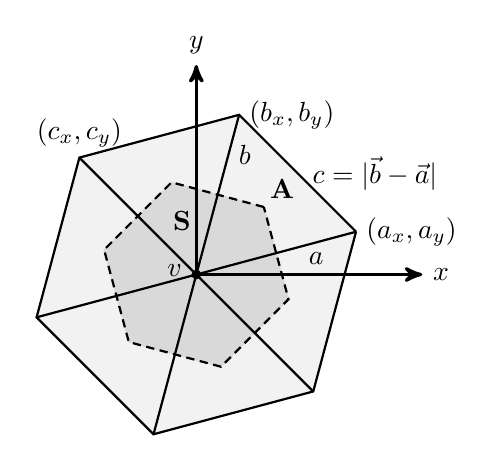
\begin{tikzpicture}[
    scale = 0.7,
    axis/.style={very thick, ->, >=stealth'},
    important line/.style={thick},
    dashed line/.style={dashed},
    pile/.style={thick, ->, >=stealth', shorten <=2pt, shorten
    >=2pt},
    every node/.style={color=black}]
    % axis
    \filldraw[fill=gray!10,draw=gray!10] (15:3) -- 
         (75:3) -- (135:3) -- (195:3) -- (255:3) -- (315:3) -- (375:3);
    \filldraw[fill=gray!30,draw=gray!30] (45:1.732)  -- (105:1.732) -- (165:1.732) -- (225:1.732) -- (285:1.732) -- (345:1.732) -- (405:1.732);
    \draw[axis] (0,0)  -- (4.1,0) node(xline)[right]{$x$};
    \draw[axis] (0,0)  -- (0,3.8) node(yline)[above]{$y$};
    \draw[thick] ( 15:-3) --node[very near end, below]{$a$} ( 15:3) node[right]{$(a_x, a_y)$};
    \draw[thick] ( 75:-3) --node[very near end, right]{$b$} ( 75:3) node[right]{$(b_x, b_y)$};
    \draw[thick] (135:-3) -- (135:3) node[above]{$(c_x, c_y)$};
    \draw[thick] (15:3) -- node[right] {\,$c=|\vec{b}-\vec{a}|$}
         (75:3) -- (135:3) -- (195:3) -- (255:3) -- (315:3) -- (375:3);
    \draw[thick] (45:2.2) node{$\mathbf{A}$} (105:1) node{$\mathbf{S}$} (170:0.4) node{$v$};
    \fill (0,0) circle (2.5pt);
    \draw[densely dashed,thick] (45:1.732)  -- (105:1.732) -- (165:1.732) -- (225:1.732) -- (285:1.732) -- (345:1.732) -- (405:1.732);
\end{tikzpicture}


\caption{\label{fig:network2continuum} 六边形单元}
\end{figure}
\end{column}
\begin{column}[c]{0.5\textwidth}
\begin{figure}[!htb]
\centering
\begin{tikzpicture}[scale = 0.7,rotate around = {15:(0,0,0)},
    axis/.style={very thick, ->, >=stealth'},
    important line/.style={thick},
    dashed line/.style={dashed, thin},
    pile/.style={thick, ->, >=stealth', shorten <=2pt, shorten
    >=2pt},
    every node/.style={color=black}]
    \coordinate (O) at (0,0);
    \coordinate (A) at (4.12,4.64);
    \coordinate (B) at (4.84,1.8);
    \coordinate (C) at (6.48,4.08);
    \coordinate (D) at (7.6,2.0);
    \coordinate (e) at (33.89:6.31);
    \coordinate (f) at (22.67:6.85);
    \coordinate (X) at ($ (B)!.625!(C) $);

    \filldraw[fill=gray!20,draw=gray!20,opacity=0.2] (O) -- (A) -- (C) -- cycle;
    \filldraw[ball color= gray!20,draw=gray!80,opacity=0.2] (O) -- (D) -- (C) -- cycle;
    \filldraw[fill=gray,draw=gray,opacity=0.2] (O) -- (B) -- (C) -- cycle;
    \draw [thick, gray] (O) -- (C) (O)-- node[near end,below]{$S$}(X); 

    \draw [very thick, dashed, black!80] (O) -- (e) (O) -- (f);
    \filldraw[fill=gray!10,draw=gray!10,opacity=0.5] (A) -- (C) -- (B) -- cycle;
    \filldraw[ball color= gray!20,draw=gray!80,opacity=0.5] (D) -- (C) -- (B) -- cycle;

    \draw[thick] (A) -- node[above] {a} (C) -- (B) -- cycle;
    
    \draw[thick] (C)-- (D) -- (B); 
    \draw[thick] (O) -- node[above]{$R$} (A) 
          (O) -- (B) 
          (O) -- node[below]{$R$} (D);
\draw[thick] (e) -- node[near start,below] {$r$} (X) (f) --  node[near start, above] {$r$} (X);
    \draw[black!80] ($ (X)!.15!(C) $) -- ($ (X)!.15!(C)!0.08!-80:(B) $) -- ($ (X)!.2!(e) $)
($ (X)!-.15!(C) $) -- ($ (X)!-.15!(C)!0.08!80:(B) $) -- ($ (X)!.19!(f) $);
    \draw [axis] (e) -- (33.89:9) node[left] {$\mathbf{n}_1$};
    \draw [axis] (f) -- (22.67:8.8) node[above] {$\mathbf{n}_2$};
    \draw (22.67:8.2)  arc(22.67:33.89:8.2) (28:8.5) node{$\theta$};
    \fill (O)    node[left]{$O$}    circle (2.5pt) 
          (33.89:6.31) circle (2pt) 
          (22.67:6.85) circle (2pt);
    \filldraw[fill=gray!20,draw=black,opacity=0.5] (O) -- (A) -- (B) -- cycle;
    \filldraw[ball color= gray!20,draw=black,opacity=0.2] (O) -- (D) -- (B) -- cycle;
\end{tikzpicture}

\vspace{-2em}
\caption{\label{fig:network2continuum} 三角形单元}
\end{figure}
\end{column}
\end{columns}
\end{frame}


\begin{frame}{细胞膜粘性}
细胞膜具有粘弹性, 传统的DPD方法不足以模拟细胞膜的粘性. 在珠簧链模型中加入$-\gamma \mathbf{v}_{ij}$项, 其表达式为
\[
\mathbf{F}_{ij}^D = 
-\bigg(
\gamma^T\mathbf{I} + \gamma^C \mathbf{e}_{ij}\mathbf{e}_{ij}
\bigg)\mathbf{v}_{ij}
=-\gamma^T\mathbf{v}_{ij} -\gamma^C(\mathbf{v}_{ij}\cdot \mathbf{e}_{ij}) \mathbf{e}_{ij}
\]
为了维持系统温度的恒定, 需要增加相应的随机力项
\[
\mathbf{F}^R_{ij} dt = \sqrt{2k_BT}
\bigg(
\sqrt{2 \gamma^T} d\overline{\mathbf{W}_{ij}^S} + \sqrt{3\gamma^C-\gamma^T}\frac{\mathrm{tr}[d\mathbf{W}_{ij}]}{3}\mathbf{I}\bigg)\mathbf{e}_{ij}
\]
其中, $d\mathbf{W}_{ij}^S$为具有独立维纳增量的对称矩阵,  $d\overline{\mathbf{W}_{ij}^S}$为相应的无迹对称矩阵. 膜的剪切粘度$\eta_m$为
\[
\eta_m=\frac{\tau_{xy}}{\dot{\gamma}} = \sqrt{3}\gamma^T+ \sqrt{3}\gamma^C/4
\]
\end{frame}

\begin{frame}
\frametitle{红细胞的运动与变形模拟: 剪切流与泊肃叶流(2D)}
\begin{columns}
\begin{column}[c]{0.5\textwidth}
\begin{figure}
\centering
\begin{overpic}[width=\textwidth]{./animate/shear2d/wall.pdf}
\put(0,0){\animategraphics[width=\textwidth, poster=first,controls,buttonsize=0.8em]{3}{./animate/shear2d/}{0}{21}}
\end{overpic}
\caption{剪切流中的红细胞}
\end{figure}
\end{column}
\begin{column}[c]{0.5\textwidth}
\begin{figure}
\centering
\begin{overpic}[width=\textwidth]{./animate/poise2d/wall.pdf}
\put(0,0){\animategraphics[width=\textwidth, poster=first,controls,buttonsize=0.8em]{3}{./animate/poise2d/}{0}{21}}
\end{overpic}
\caption{泊肃叶流中的红细胞}
\end{figure}
\end{column}
\end{columns}
\end{frame}

\begin{frame}{细胞膜粘附模型}
\begin{center}
\includegraphics[width=\textwidth]{adhesion.pdf}
\end{center}
\end{frame}

\begin{frame}{细胞膜粘附模型}
配体(细胞膜上的粒子)和受体(壁面上的粒子)间形成bond
\[
F(l) = k_s(l-l_0)
\]
形成bond和断裂bond的概率分别为
\[
P_{on}=\begin{cases}
1-\mathrm{e}^{-k_{\mathrm{on}}\Delta t} & l<d_{\mathrm{on}}\\
0 & l\geq d_{\mathrm{on}}
\end{cases},\quad P_{\mathrm{off}}=\begin{cases}
1-\mathrm{e}^{-k_{\mathrm{off}}\Delta t} & l<d_{off}\\
1 & l\geq d_{\mathrm{off}}
\end{cases}
\]
其中
\[
k_{\mathrm{on}} = k_{\mathrm{on}}^0\exp\bigg(-\frac{\sigma_{\mathrm{on}}(l-l_0)^2}{2k_BT}\bigg),\quad
k_{\mathrm{off}} = k_{\mathrm{off}}^0\exp\bigg(-\frac{\sigma_{\mathrm{off}}(l-l_0)^2}{2k_BT}\bigg)
\]

\end{frame}


\begin{frame}{三维红细胞的拉伸}
\begin{columns}
\begin{column}[c]{0.5\textwidth}
\begin{center}
%\pgfplotsset{compat=1.6}
\newcommand{\rbc}[2]{
\begin{tikzpicture}
\begin{axis}[xmin=-8.5,xmax=8.5,ymin=-4.5,ymax=4.5,width=\textwidth,height=0.8\textwidth,
xticklabel style={font=\scriptsize},
yticklabel style={font=\scriptsize},
xlabel style={font=\footnotesize},
ylabel style={font=\footnotesize},
xlabel={force = #2 pN},
colormap={bw}{gray(0cm)=(0); gray(1cm)=(1)}, view={0}{90},axis equal]
\addplot3[patch] file{./animate/stretch/data/#1};
\end{axis}

\begin{axis}[yshift=-0.55\textwidth,xmin=-8.5,xmax=8.5,zmin=-3,zmax=3,width=\textwidth,height=0.6\textwidth,
zticklabel style={font=\scriptsize},
xticklabel style={font=\scriptsize},
xlabel style={font=\footnotesize},
zlabel style={font=\footnotesize},
colormap={bw}{gray(0cm)=(0); gray(1cm)=(1)}, view={0}{0}, axis equal]
\addplot3[patch] file{./animate/stretch/data/#1};
\end{axis}
\end{tikzpicture}
}

\begin{animateinline}[autoplay,poster=last,controls,buttonsize=0.8em]{3}
%\rbc{2-1txt}{0}\newframe
%\rbc{2-11txt}{20}\newframe
%\rbc{4-11txt}{40}\newframe
%\rbc{6-11txt}{60}\newframe
%\rbc{8-11txt}{80}\newframe
%\rbc{10-11txt}{100}\newframe
%\rbc{12-11txt}{120}\newframe
%\rbc{14-11txt}{140}\newframe
%\rbc{16-11txt}{160}\newframe
%\rbc{18-11txt}{180}\newframe
\rbc{20-11txt}{200}
\end{animateinline}

\animategraphics[width=\textwidth,poster=first,controls,buttonsize=0.8em,autoplay,loop]{2}{./animate/stretch/}{0}{10}
\end{center}

\end{column}
\begin{column}[c]{0.5\textwidth}
\begin{tikzpicture}[scale=0.925]
\begin{axis}[xmin=0,xmax=200,ymin=0,ymax=22,width=182pt,height=1.44\textwidth,xlabel={force ($\mathrm{pN}$)},ylabel={diameter ($\mathrm{\mu m}$)},
ytick={0,2,...,20},
label style={anchor=near ticklabel},
    ylabel style={yshift=-2em},
    xlabel style={yshift=0.3em},
    tick label style={font=\scriptsize },
    label style={font=\footnotesize},
    legend style={font=\tiny,legend cell align=left,legend pos=north west}
]


\addplot+[mark=diamond,only marks,error bars/.cd,
	y dir=both,y explicit]
coordinates {
(  0.01,  7.820) +- (0,0.780)
( 16.41,  9.230) +- (0,0.880)
( 19.70,  9.535) +- (0,0.935)
( 31.01, 10.455) +- (0,0.955)
( 38.30, 11.145) +- (0,1.145)
( 47.11, 11.870) +- (0,1.090)
( 67.51, 12.860) +- (0,1.070)
( 87.60, 13.775) +- (0,1.225)
(108.99, 14.390) +- (0,1.470)
(130.01, 15.190) +- (0,1.450)
(151.01, 15.610) +- (0,1.300)
(173.00, 16.065) +- (0,1.815)
(192.99, 16.255) +- (0,1.795)
(  0.01,  7.515) +- (0,0.705)
( 16.41,  6.195) +- (0,0.665)
( 19.70,  6.260) +- (0,0.710)
( 31.01,  5.760) +- (0,0.570)
( 38.30,  5.405) +- (0,0.595)
( 47.11,  5.090) +- (0,0.820)
( 67.51,  4.695) +- (0,0.735)
( 87.60,  4.665) +- (0,0.635)
(108.99,  4.595) +- (0,0.715)
(130.01,  4.575) +- (0,0.635)
(151.01,  4.405) +- (0,0.605)
(173.00,  4.580) +- (0,0.510)
(192.99,  4.395) +- (0,0.615)};

\addlegendentry{Experiment}

\addplot+[no marks,red,smooth] table[x=x,y=y]{./figures/data/spectrin.dat};
\addlegendentry{spectrin-level, Dao et al.}

\addplot+[no marks,black,densely dashed,smooth,thick] table[x=f,y=w]{./figures/data/wlc-pow.dat};
\addlegendentry{wlc-pow, $N_v = 500$}

\addplot+[no marks,black,densely dotted,smooth,thick] table[x=f,y=w]{./figures/data/fene-pow.dat};
\addlegendentry{fene-pow, $N_v = 500$}

\node[font=\footnotesize] at (axis cs:170,7){$D_T$};
\node[font=\footnotesize] at (axis cs:170,12.5){$D_A$};

\end{axis}
\end{tikzpicture}

\vspace{-2.6em}
\end{column}
\end{columns}
\end{frame}

\begin{frame}{剪切流中的三维红细胞, $\dot{\gamma}=10 \mathrm{s}^{-1}$}
\begin{columns}
\begin{column}[c]{0.5\textwidth}
\begin{center}
\animategraphics[width=\textwidth,poster=first,controls,buttonsize=0.8em,autoplay,loop]{5}{./animate/shear10/}{1}{71}
\end{center}
\end{column}
\begin{column}[c]{0.5\textwidth}
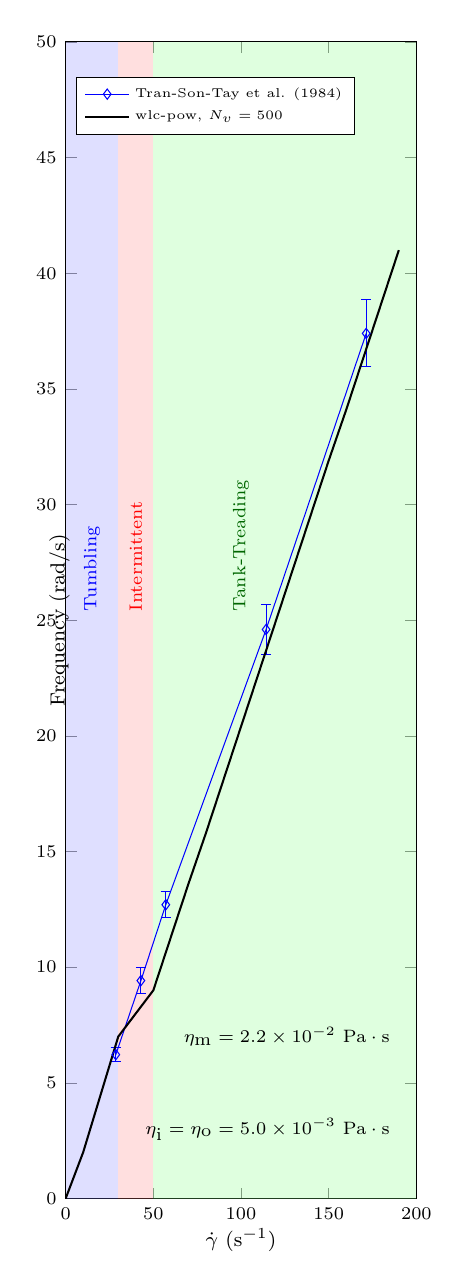
\begin{tikzpicture}[scale=0.925]
\begin{axis}[xmin=0,xmax=200,ymin=0,ymax=50,width=182pt,height=1.44\textwidth,
xlabel={$\dot{\gamma}$ ($\mathrm{s}^{-1}$)},ylabel={Frequency ($\mathrm{rad/s}$)},
label style={anchor=near ticklabel},
    ylabel style={yshift=-2em},
    xlabel style={yshift=0.3em},
    tick label style={font=\scriptsize },
    label style={font=\footnotesize},
legend style={font=\tiny,legend cell align=left,legend pos=north west}
]

\fill[blue!50,opacity=0.25] (axis cs:0,0)--(axis cs:30,0)--(axis cs:30,50)--(axis cs:0,50)--cycle;
\fill[red!50,opacity=0.25] (axis cs:30,0)--(axis cs:50,0)--(axis cs:50,50)--(axis cs:30,50)--cycle;
\fill[green!50,opacity=0.25] (axis cs:50,0)--(axis cs:200,0)--(axis cs:200,50)--(axis cs:50,50)--cycle;
\addplot+[mark=diamond,error bars/.cd,
	y dir=both,y explicit]
coordinates {
(28.6, 6.22) +- (0,0.31)
(42.9, 9.42) +- (0,0.57)
(57.1,12.70) +- (0,0.57)
(114.3,24.6) +- (0,1.07)
(171.4,37.4) +- (0,1.45)};

\addlegendentry{Tran-Son-Tay et al. (1984)};

\addplot+[no marks,thick,black] table[x=x,y=y]
{x    y
 0    0
 10   2   
 20   4.5
 30   7
 40   8
 50   9
 60   11.3
 70   13.6
 80   15.8
 90   18.1
100   20.4
110   22.7
120   25
130   27.3
140   29.6
150   31.9
160   34.1
170   36.4
180   38.7
190   41
};
\addlegendentry{wlc-pow, $N_v=500$}


\node[font=\scriptsize,left] at (axis cs:190,3){$\eta_{\textrm{i}} = \eta_{\textrm{o}} = 5.0\times 10^{-3}~ \mathrm{Pa\cdot s}$};
\node[font=\scriptsize,left] at (axis cs:190,7){$\eta_{\textrm{m}} = 2.2\times 10^{-2}~\mathrm{Pa\cdot s}$};


\node[font=\scriptsize,right,rotate=90,blue] at (axis cs:15,25){Tumbling};
\node[font=\scriptsize,right,rotate=90,red] at (axis cs:40,25){Intermittent};
\node[font=\scriptsize,right,rotate=90,green!40!black] at (axis cs:100,25){Tank-Treading};
\end{axis}
\end{tikzpicture}

\vspace{-2.6em}
\end{column}
\end{columns}
\end{frame}

\begin{frame}{剪切流中的三维红细胞, $\dot{\gamma}=30 \mathrm{s}^{-1}$}
\begin{columns}
\begin{column}[c]{0.5\textwidth}
\begin{center}
\animategraphics[width=\textwidth,poster=first,controls,buttonsize=0.8em,autoplay,loop]{5}{./animate/shear30/}{1}{59}
\end{center}
\end{column}
\begin{column}[c]{0.5\textwidth}
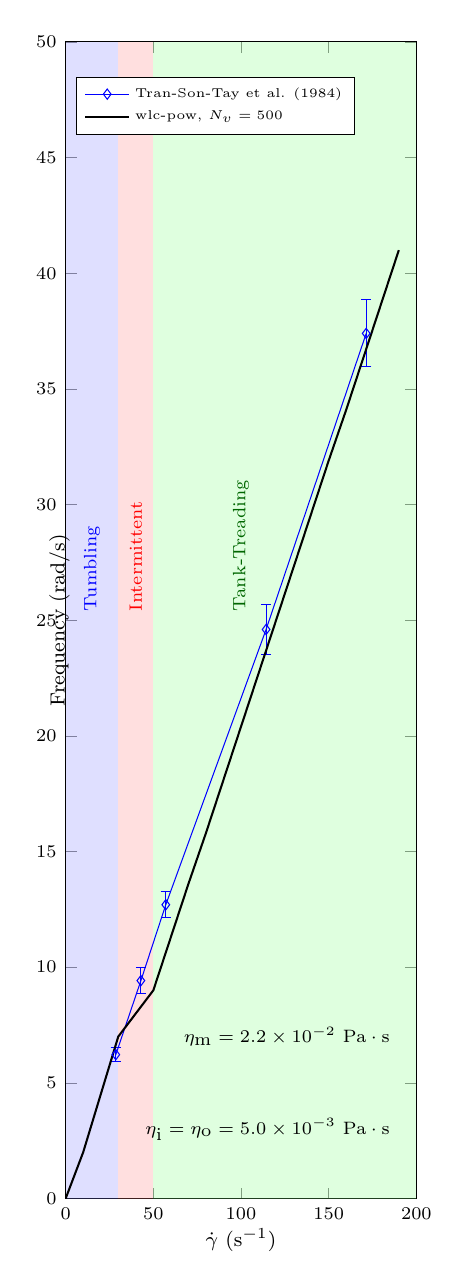
\begin{tikzpicture}[scale=0.925]
\begin{axis}[xmin=0,xmax=200,ymin=0,ymax=50,width=182pt,height=1.44\textwidth,
xlabel={$\dot{\gamma}$ ($\mathrm{s}^{-1}$)},ylabel={Frequency ($\mathrm{rad/s}$)},
label style={anchor=near ticklabel},
    ylabel style={yshift=-2em},
    xlabel style={yshift=0.3em},
    tick label style={font=\scriptsize },
    label style={font=\footnotesize},
legend style={font=\tiny,legend cell align=left,legend pos=north west}
]

\fill[blue!50,opacity=0.25] (axis cs:0,0)--(axis cs:30,0)--(axis cs:30,50)--(axis cs:0,50)--cycle;
\fill[red!50,opacity=0.25] (axis cs:30,0)--(axis cs:50,0)--(axis cs:50,50)--(axis cs:30,50)--cycle;
\fill[green!50,opacity=0.25] (axis cs:50,0)--(axis cs:200,0)--(axis cs:200,50)--(axis cs:50,50)--cycle;
\addplot+[mark=diamond,error bars/.cd,
	y dir=both,y explicit]
coordinates {
(28.6, 6.22) +- (0,0.31)
(42.9, 9.42) +- (0,0.57)
(57.1,12.70) +- (0,0.57)
(114.3,24.6) +- (0,1.07)
(171.4,37.4) +- (0,1.45)};

\addlegendentry{Tran-Son-Tay et al. (1984)};

\addplot+[no marks,thick,black] table[x=x,y=y]
{x    y
 0    0
 10   2   
 20   4.5
 30   7
 40   8
 50   9
 60   11.3
 70   13.6
 80   15.8
 90   18.1
100   20.4
110   22.7
120   25
130   27.3
140   29.6
150   31.9
160   34.1
170   36.4
180   38.7
190   41
};
\addlegendentry{wlc-pow, $N_v=500$}


\node[font=\scriptsize,left] at (axis cs:190,3){$\eta_{\textrm{i}} = \eta_{\textrm{o}} = 5.0\times 10^{-3}~ \mathrm{Pa\cdot s}$};
\node[font=\scriptsize,left] at (axis cs:190,7){$\eta_{\textrm{m}} = 2.2\times 10^{-2}~\mathrm{Pa\cdot s}$};


\node[font=\scriptsize,right,rotate=90,blue] at (axis cs:15,25){Tumbling};
\node[font=\scriptsize,right,rotate=90,red] at (axis cs:40,25){Intermittent};
\node[font=\scriptsize,right,rotate=90,green!40!black] at (axis cs:100,25){Tank-Treading};
\end{axis}
\end{tikzpicture}

\vspace{-2.6em}
\end{column}
\end{columns}
\end{frame}

\begin{frame}{剪切流中的三维红细胞, $\dot{\gamma}=100 \mathrm{s}^{-1}$}
\begin{columns}
\begin{column}[c]{0.5\textwidth}
\begin{center}
\animategraphics[width=\textwidth,poster=first,controls,buttonsize=0.8em,autoplay,loop]{5}{./animate/shear/}{0}{70}
\end{center}
\end{column}
\begin{column}[c]{0.5\textwidth}
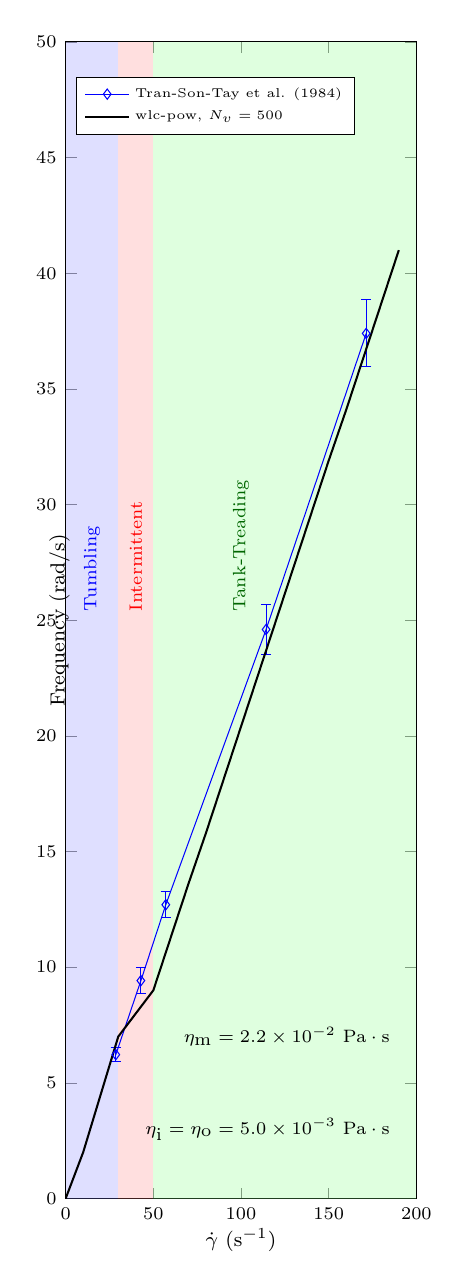
\begin{tikzpicture}[scale=0.925]
\begin{axis}[xmin=0,xmax=200,ymin=0,ymax=50,width=182pt,height=1.44\textwidth,
xlabel={$\dot{\gamma}$ ($\mathrm{s}^{-1}$)},ylabel={Frequency ($\mathrm{rad/s}$)},
label style={anchor=near ticklabel},
    ylabel style={yshift=-2em},
    xlabel style={yshift=0.3em},
    tick label style={font=\scriptsize },
    label style={font=\footnotesize},
legend style={font=\tiny,legend cell align=left,legend pos=north west}
]

\fill[blue!50,opacity=0.25] (axis cs:0,0)--(axis cs:30,0)--(axis cs:30,50)--(axis cs:0,50)--cycle;
\fill[red!50,opacity=0.25] (axis cs:30,0)--(axis cs:50,0)--(axis cs:50,50)--(axis cs:30,50)--cycle;
\fill[green!50,opacity=0.25] (axis cs:50,0)--(axis cs:200,0)--(axis cs:200,50)--(axis cs:50,50)--cycle;
\addplot+[mark=diamond,error bars/.cd,
	y dir=both,y explicit]
coordinates {
(28.6, 6.22) +- (0,0.31)
(42.9, 9.42) +- (0,0.57)
(57.1,12.70) +- (0,0.57)
(114.3,24.6) +- (0,1.07)
(171.4,37.4) +- (0,1.45)};

\addlegendentry{Tran-Son-Tay et al. (1984)};

\addplot+[no marks,thick,black] table[x=x,y=y]
{x    y
 0    0
 10   2   
 20   4.5
 30   7
 40   8
 50   9
 60   11.3
 70   13.6
 80   15.8
 90   18.1
100   20.4
110   22.7
120   25
130   27.3
140   29.6
150   31.9
160   34.1
170   36.4
180   38.7
190   41
};
\addlegendentry{wlc-pow, $N_v=500$}


\node[font=\scriptsize,left] at (axis cs:190,3){$\eta_{\textrm{i}} = \eta_{\textrm{o}} = 5.0\times 10^{-3}~ \mathrm{Pa\cdot s}$};
\node[font=\scriptsize,left] at (axis cs:190,7){$\eta_{\textrm{m}} = 2.2\times 10^{-2}~\mathrm{Pa\cdot s}$};


\node[font=\scriptsize,right,rotate=90,blue] at (axis cs:15,25){Tumbling};
\node[font=\scriptsize,right,rotate=90,red] at (axis cs:40,25){Intermittent};
\node[font=\scriptsize,right,rotate=90,green!40!black] at (axis cs:100,25){Tank-Treading};
\end{axis}
\end{tikzpicture}

\vspace{-2.6em}
\end{column}
\end{columns}
\end{frame}


\begin{frame}{多个红细胞管道流动}
\includegraphics[width=\textwidth]{./figures/rbc.png}
\end{frame}
